\documentclass[UTF8]{ctexart}
\usepackage{amsmath}
\usepackage{amssymb}
\usepackage{background}
\usepackage{caption, subcaption}
\usepackage{circuitikz}
\usepackage{enumitem}
\usepackage{float}
\usepackage{fourier}
\usepackage{fontspec}
\usepackage{geometry}
\usepackage{pifont}
\usepackage{tikz}
\usepackage{ulem}
\usepackage{xcolor}
\usetikzlibrary{arrows.meta}



%\backgroundsetup{contents=
\includegraphics{示例.png}, center, scale=1, angle=0, opacity=1}
\geometry{a5paper, top=0.1cm, left=1cm, right=1cm, bottom=1.1cm}
\setCJKmainfont[BoldFont={汉仪文黑-85W},ItalicFont={方正苏新诗柳楷简体}]{汉仪文黑-55W}
\setfontfamily\Issue{Century Schoolbook}
\newCJKfontfamily\TitleFont{思源宋体 CN Heavy}
\newfontfamily\timesnewroman{Times New Roman}
\captionsetup{font=small, labelfont=bf}


\newcommand\Black[1]{\textcolor[gray]{0.3}{#1}}
\newcommand\Brown[1]{\textcolor[HTML]{998A4E}{#1}}
\newcommand\Emph[1]{\colorbox{red!20!}{\textcolor{red!80!black}{#1}}}
\newcommand\Correct[1]{\colorbox{green!20}{\textcolor{green!50!black}{#1}}}
\newcommand\mypi{\text{\timesnewroman π}}
%这4个信息随“刊号”更新
\newcommand\IssueNumber{04}
\newcommand\Date{2023-10-12}
%\newcommand\Contributer{@金光日}
\newcommand\Subject{模拟电子线路}
\renewcommand\thefootnote{\ding{\numexpr171 + \value{footnote}}}
\newcommand\xb[1]{_\mathrm{#1}}

\ctikzset{resistors/scale=0.6, % smaller R
    capacitors/scale=0.7, % even smaller C
    diodes/scale=0.6, % small diodes
    transistors/scale=1.3,
    sources/scale=0.6,
}


\begin{document}
\backgroundsetup{contents=
\includegraphics{上半示例.png}, center, scale=1, angle=0, opacity=1}
\BgThispage
\begin{center}
{\scriptsize\Issue \textcolor[HTML]{C8BA83}{WEEKLY TIPS}}

{\Huge\bfseries\TitleFont \Black{知\ 识\ 小\ 料}}

\vspace{-0.1cm}
{\footnotesize \Brown{「电计 2203 班」周常规知识整理共享}}
\end{center}

\vspace{-0.5cm}

\begin{figure}[H]
\hspace{1cm}
\begin{minipage}[t]{0.3\textwidth}
\centering
    \Brown{ISSUE.}

    \vspace{-0.6cm}
    \Huge \Issue\slshape\bfseries\Black{\IssueNumber}
\end{minipage}
\hfill
\begin{minipage}[t]{0.3\textwidth}
\centering
    \Brown{日期:\Date} \\
%\vspace{-0.1cm}
%    \Brown{贡献者:\Contributer} \\
\vspace{-0.1cm}
    \Brown{学科:\Subject} \\
\end{minipage}
\hspace{0.8cm}
\end{figure}

%此处以后填写正文

{\color{cyan!50!black}
两级电压放大电路如图所示。已知 $\mathrm{T_1}$ 的 $I\xb{D1} = \mathrm{1mA}$,$g\xb{m1} = \mathrm{3mS}$,$\mathrm{T_2}$ 的 $\beta = 100$,$r\xb{bb'} = \mathrm{200\Omega}$,$V\xb{BE}=\mathrm{0.6V}$。在信号中频频率范围,各电容容抗均可忽略。(共 24 分)

\begin{enumerate}[itemsep=0pt, parsep=0pt]
  \item $\mathrm{T_1}$ 和 $\mathrm{T_2}$ 分别构成了什么组态电路?(2 分)
  \item 计算 $\mathrm{T_1}$、$\mathrm{T_2}$ 的静态工作点:$V\xb{GS1}$、$V\xb{DS1}$,$I\xb{C2}$、$V\xb{CE2}$;(8 分)
  \item 计算该电路的输入电阻 $R\xb{i}$ 和输出电阻 $R\xb{o}$;(5 分)
  \item 计算该电路的电压放大倍数 $A_v$。(9 分)
\end{enumerate}

\begin{figure}[ht]
  \centering
  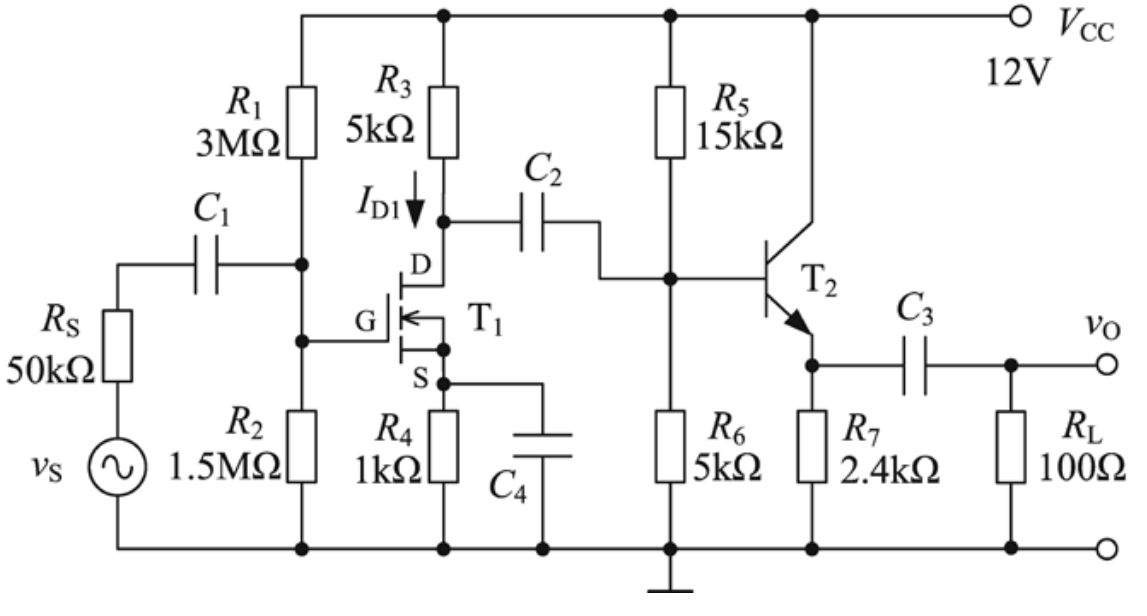
\includegraphics[width=10cm]{题图.png}
\end{figure}
}

\noindent 【第 1 小问】 $\mathrm{T_1}$ 栅极输入、漏极输出,因此为\uline{共源极放大电路};$\mathrm{T_2}$ 基极输入,发射极输出,因此为\uline{共集电极放大电路}。\textcolor{cyan}{(果不其然,共集电极真的很常考。)}

\noindent 【第 2 小问】先求 $\mathrm{T_1}$,这算是一种分压式偏置电路,已知 $I\xb{D1}=\mathrm{1mA}$。

$V\xb{G} = V\xb{CC}\cdot\frac{R_2}{R_1+R_2} = \mathrm{4V}$

$V\xb{S} = I\xb{D1}R_4 = \mathrm{1V}$

$V\xb{GS1} = V\xb{G} - V\xb{S} = \uline{\mathrm{3V}}$

$V\xb{DS1} = V\xb{CC} - I\xb{D1}(R_3+R_4) = \uline{\mathrm{6V}}$ \textcolor{cyan}{($I\xb{D1}$ 通流两个电阻)}

接下来求 $\mathrm{T_2}$,典型的「双 $R\xb{b}$ 偏置电路」。注意本题 $V\xb{BE}$ 是 0.6V。

$V\xb{B} = V\xb{CC}\cdot \frac{R_6}{R_5+R_6} = \mathrm{3V}$

\newpage
\backgroundsetup{contents=
\includegraphics{下半示例.png}, center, scale=1, angle=0, opacity=1}
\BgThispage
\phantom{...}
\vspace{0.5cm}

$I\xb{C2} = \frac{V\xb{B}-V\xb{BE}}{R_7} = \uline{\mathrm{1mA}}$\textcolor{cyan}{(不可以忽略 $V\xb{BE}$ 的影响)}

$V\xb{CE2} = V\xb{CC} - I\xb{C2}R_7 = \uline{\mathrm{9.6V}}$

\noindent 【第 3 小问】接下来是动态分析,推荐画出小信号等效电路后再往下看。

总输入电阻是 $\mathrm{T_1}$ 的输入电阻,为 $R\xb{i} = R_1 \parallel R_2 = \uline{\mathrm{1M\Omega}}$

总输出电阻是 $\mathrm{T_2}$ 的输出电阻,而共集电极的输出电阻为
\begin{equation}
    R\xb{o} = R_7\parallel \dfrac{r\xb{be} + (R_5\parallel R_6)\parallel R\xb{s2}}{1+\beta}
\end{equation}
注意这里涉及到一个 $R\xb{s2}$,表示对 $\mathrm{T_2}$ 而言的「电源」内阻。而由共集电极特有的「级间影响」,应有 \Emph{$R\xb{s2} = R\xb{o1}$} $= R_3 = \mathrm{5k\Omega}$。

加上一个 $r\xb{be} = r\xb{bb'}+(1+\beta)\frac{\mathrm{26mV}}{I\xb{E2}} = \mathrm{2.8k\Omega}$,我们可以求出
\begin{equation}
    R\xb{o} = \mathrm{2.4k \parallel \dfrac{2.8k + (15k\parallel 5k)\parallel 5k}{101} \approx \uline{48\Omega}}
\end{equation}

\noindent 【第 4 小问】$A_v = A_{v1} A_{v2}$。\textcolor{cyan}{(先写上得 1 分。)}

对于共源极电路,$A_{v1} = -g\xb{m}(R_3\parallel R\xb{L1})$,而又由「级间影响」,\Emph{$R\xb{L1} = R\xb{i2}$},也就是共集电极电路的输入电阻。
\begin{equation}
    R\xb{i2} = (R_5\parallel R_6) \parallel [r\xb{be} + (1+\beta)(R_7\parallel R\xb{L})] \approx \mathrm{2.9k\Omega}
\end{equation}
故 $A_{v1} = -g\xb{m}(R_3\parallel R\xb{L1}) \approx -5.4$。

对于共集电极电路,我们有
\begin{equation}
    A_{v2} = \dfrac{(1+\beta)(R_7\parallel R\xb{L})}{r\xb{be} + (1+\beta)(R_7\parallel R\xb{L})} \approx 0.77
\end{equation}

因此 $A_v = -5.4\times 0.77 \approx \uline{-4.16}$。

\textcolor{cyan!80!black}{(注:画线的部分代表计算结果;因为不可获取标准答案,计算结果可能与标准答案存在一定误差。)}

\textcolor{cyan!80!black}{【点评】本题是一道典型的多级放大问题,考察了常见的静动态分析问题,而且把共集电极电路的 $A_v$、$R\xb{i}$、$R\xb{o}$ 都考了一遍。共集电极电路和「级间影响」是常考点,同学们应多多留意。}

\end{document} 